\chapter{Matrix III: Eigenvalue Problems}\label{ch:matrix3}

In Chapter \ref{ch:ode3} we studied eigenvalue problems in ODE. Eigenvalue problems can be expressed  also in matri: 
\begin{equation}\label{eq:general_eigen}
   A \mathbf{u} = \lambda \mathbf{u}
\end{equation}
where $\lambda$ is an eigenvalue and $\mathbf{u}$ is the eigenvector corresponding to the eigenvalue. 
The matrix $A$ can be real or complex.  Even when $A$ is real, the eigenvalues can be complex.   When the matrix is self-adjoint ($A^\dagger=A$) the eigenvalues are all real.   The eigenvalue problem of a complex self-adjoint matrix can be converted to an eigenvalue problem of a symmetric real matrix.  Consider a self-adjoint matrix $A = B + iC$ where $B$ ans $C$ are real matrices.
Its adjoint is $A^\dagger = B^\textsc{t} - i C^\textsc{T}$.   Since $A$ is self-adjoint, $B$ is symmetric ($B^\textsc{t}=B$) and $C$ is anti-symmetric ($C^\textsc{t}=-C$).  Writing the eigenvalues in $\mathbf{u}=\mathbf{x}+i \mathbf{y}$ where $\mathbf{x}$ and $\mathbf{y}$ are real vectors, the original eigenvalue problem is transformed to an eigenvalue problem of real symmetric matrix:
\begin{equation}\label{eq:complex_eqigen}
\begin{bmatrix} B & -C \\ C & B \end{bmatrix} 
\begin{bmatrix} \mathbf{x} \\ \mathbf{y} \end{bmatrix}
= \lambda
\begin{bmatrix} \mathbf{x} \\ \mathbf{y} \end{bmatrix}\,.
\end{equation}
In this chapter, we focus only on real symmetric  matrices.

In some cases we want to find all eigenvalues and in other cases we are interested in only the lowest eigenvalue. For each case, there are suitable numerical algorithms.  In this chapter we discuss some of them which work well for relatively small problems.  For very large matrices, there are more complicated algorithms which are not covered in this lecture.

\section{The Power Method}

We begin with a simple iterative method which converges to an eigenvalue whose absolute value is the largest among all eigenvalues. Consider an eigenvalue problem of $N$ dimension:
\begin{equation}
A \mathbf{u}_n = \lambda_n \mathbf{u}_n,\qquad n=1,\cdots, N
\end{equation}
with eigenvalues $\lambda_n$ ordered as
\begin{equation}\label{eq:lambda_order}
|\lambda_1| > |\lambda_2| \geq \cdots \geq |\lambda_{N-1}| \geq |\lambda_N|\,.
\end{equation}
Note that $\lambda_1$ is strictly larger than $\lambda_2$ and no degeneracy is allowed between them.  This is not a severe restriction. We will discuss how to resolve degeneracy later.  The eigenvector $\mathbf{u}_n$ is assumed to be normalized.

Th iterative process starts with a normalized random vector $\mathbf{x}^{(0)}$ which is expanded as
\begin{equation}
\mathbf{x}^{(0)}= \sum_{n=1}^N c_n \mathbf{u}_n
\end{equation}
where $c_n$ is an expansion coefficient.  We assume that $c_1 \ne 0$.  Since we do know the eigenvectors yet.  We have no way to guarantee it.
We hope that the random vector will not accidentally orthogonal to $\mathbf{u}_1$.  Multiplying $A$ to $\mathbf{x}^{(0)}$ leads to
\begin{equation}
A \mathbf{x}^{(0)} = A \sum_n c_n \mathbf{u}_n = \sum_n c_n A \mathbf{u}_n = \sum_n c_n \lambda_n \mathbf{u}_n
\end{equation}
and after repeating it $m$ times we obtain
\begin{equation}
A^m \mathbf{x}^{(0)} = \sum_n c_n \lambda_n^m \mathbf{u}_n= \lambda_1^m \left [ c_1 \mathbf{u}_1 + \sum_{n=2}^N c_n \left ( \frac{\lambda_n}{\lambda_1} \right )^m
\mathbf{u}_n \right ]
\end{equation}
Noting that $|\lambda_n/\lambda_1|<1$ for $n\geq 2$, $|\lambda_n/\lambda_1|^m$ vanishes as $m \rightarrow \infty$.  Then, the dominant term and its norm are given by
\begin{equation}\label{eq:eigen_power}
A^m \mathbf{x}^{(0)} \xrightarrow[m \rightarrow \infty]{} c_1 \lambda_1^m \mathbf{u}_1
\end{equation}
and
\begin{equation}\label{eq:eqigen_power_norm}
\| A^m \mathbf{x}^{(0)}\| \xrightarrow[m \rightarrow \infty]{} |c_1| |\lambda_1|^m \|\mathbf{u}_1\|\,.
\end{equation}
These equations still contain an unknown quantity $c_1$, which is eliminated by taking the ratio of these equations.  The ratio now converges to the eigenvector up to the phase factor: 
\begin{equation}
\mathbf{x}^{(m)} \equiv \frac{A^m \mathbf{x}^{(0)}}{\|A^{m}\mathbf{x}^{(0)}\|} \quad
\xrightarrow[m \rightarrow \infty]{} \quad
\frac{c_1 \lambda_1^m \mathbf{u}_1}{|c_1| |\lambda_1|^m \|\mathbf{u}_1\|} 
= \mathbf{u}_1\,.
\end{equation}
We can safely ignore the phase factor which is arbitrary in eigenvalue problems. (If $\mathbf{u}$ is a solution, so is $\me^{i \phi} \mathbf{u}$.).   It is also noted that the final result is automatically normalized. 
Once we found the eigenvector $\mathbf{u}_1$, the corresponding eigenvalue can be computed by
\begin{equation}
\lambda_1 = (\mathbf{x}^{(m)})^\textsc{t} A \mathbf{x}^{(m)}\,.
\end{equation}

The above iterative procedure is known as the power method for the ``largest'' eigenvalue in the sense of Eq. ({\ref{eq:lambda_order}).
If we want to find the smallest eigenvalue $\lambda_N$, there is a trick to get it using the power method.  We invert the original equation as follows:
\begin{equation}
A \mathbf{u} = \lambda \mathbf{u} \quad \Longrightarrow \quad A^{-1} \mathbf{u} = \lambda^{-1} \mathbf{u}.
\end{equation}
Let $B=A^{-1}$ and $\eta=\lambda^{-1}$ and solve $B \mathbf{u}=\eta \mathbf{u}$ by the power method.  We will get the largest eigenvalue $\eta$ which is the smallest in the original expression $\lambda_N=1/\eta$.  

For other eigenvalues, we have another trick.  First, we guess an eigenvalue $\lambda^\prime$ and then subtract $\lambda^\prime \mathbf{u}$ from both sides of the original equation. The resulting equation is again an eigenvalue problem:
\begin{equation}
(A - \lambda^\prime I) \mathbf{u} = (\lambda-\lambda^\prime) \mathbf{u}
\end{equation}
where $I$ represents an identity matrix.  Letting $B=A-\lambda^\prime I$ and $\eta=\lambda-\lambda^\prime$, we are solving another eigenvalue equation: $B\mathbf{u}=\eta \mathbf{u}$.  If we use the power method for the smallest eigenvalue,  the resulting eigenvalue $\eta$ is the smallest.  Transforming back to the original eigenvalue we have $\lambda = \lambda^\prime + \eta$.  Since $\eta$ is the smallest, we found an eigenvalue closest to $\lambda^\prime$. This method fails when the initial guess is too close to an eigenvalue since $\mathbf{x}^{(m)}$ diverges.  If we should get a huge $\mathbf{x}^{(m)}$,  change the value of $\lambda^\prime$.

For any iterative method, there must be a condition to stop the procedure. If a bad condition is used, the process may falls into an endless loop.  A typical condition is if a quantity changes significantly by a step of the iteration. Since we update
the vector $\mathbf{x}^{(m)}$, it is a good quantity to check.
So, we compare $\mathbf{x}^{(n)}$ and $\mathbf{x}^{(n-1)}$.  Typically the norm of the difference between two vectors 
\begin{equation}\label{eq:x_improve}
\|\mathbf{x}^{(n)}- \mathbf{x}^{(n-1)}\|
\end{equation}
is used as the measure of error.  If this quantity is smaller than a tolerance, we stop the iteration.
However, this method may fail in the present procedure.  During the iterations the sign of the vector may flip. The sign of the eigenvector is not significant. Both $\mathbf{x}^{(n)}$ and $-\mathbf{x}^{(n)}$ are equally good candidates for the eigenvector although they are two different vectors.  However, Eq. (\ref{eq:x_improve}) is not a small quantity when the sign flips.  Therefore, we have to make it sure that the iteration does not flip the sign of $\mathbf{x}$. If the sign flipped, we just need to flip back the sign.  See the Algorithm shown in the following box.

\bigskip
\begin{samepage}
\begin{center}
\Algorithm{Power method for the largest eigenvalue}
\fbox{\colorbox{cream}{
\begin{minipage}{5in}
\begin{enumerate}
\item Pick a normalized random vector $\mathbf{x}^{(0)}$.
\item Repeat the following iterative procedure starting with $n=1$.
\item Calculate a new vevtor: $\mathbf{y} = A \mathbf{x}^{(n-1)}$.
\item Normalize the vector: $\mathbf{x}^{(n)} = \displaystyle\frac{\mathbf{y}}{\|\mathbf{y}\|}$.
\item If $x_1^{(n)}<0$, then reverse the sign of the vector: $\mathbf{x}^{(n)} = -\mathbf{x}^{(n)}$.
\item If $\|\mathbf{x}^{(n)}- \mathbf{x}^{(n-1)}\| < \text{tolerance}$, then and $\mathbf{x}^{(n)}$ is the eigenvector.  Otherwise increment $n$ and go to step 3.
\item Calculate the eigenvalue $\lambda =  \left ( \mathbf{x}^{(n)}\right )^\textsc{t} A \mathbf{x}^{(n)}$.
\end{enumerate}
\end{minipage}
}}
\end{center}
\end{samepage}


\bigskip
\begin{example}\label{ex:eigen_power_large}

We first calculate the largest eigenvalue of 
\begin{equation}
A=
\begin{bmatrix}
2 & 1 & 0 \\ 1 & 2 & 1\\ 0 & 1 & 2
\end{bmatrix}
\end{equation}
using the power method.   Try a random initial vector $\mathbf{x}_0$.  Then, try another initial vector $\mathbf{x}_0 = [2, -\sqrt{2}, 0]^\textsc{t}$.

The exact eigenvalues of this matrix is $\lambda_1=2+\sqrt{2}=3.4142135$, $\lambda_2=2$, and $\lambda_3=2-\sqrt{2}=0.585786$. The corresponding eigenvectors are
\begin{equation}
\mathbf{u}_1 = \begin{bmatrix}
1/2 \\ 1/\sqrt{2} \\ 1/2
\end{bmatrix}, \qquad
\mathbf{u}_2 = \begin{bmatrix}
1\sqrt{2} \\ 0 \\ -1/\sqrt{2}
\end{bmatrix}, \qquad
\mathbf{u}_1 = \begin{bmatrix}
1/2 \\ -1/\sqrt{2} \\ 1/2
\end{bmatrix}
\end{equation}

Program \ref{prog:power_eigen} implements the power method and find the eigenvalue and eigenvector.
Starting with a random vector, the power method iterated 26 times with the tolerance=$1\times 10^{-7}$ and converged to a large eigenvelue 3.414214, in good agreement with the exact value.  The eigenvector $[0.500000, 0.707107, 0.500000]^\textsc{t}$ also agrees well.  However, when the other initial vector $[2, \sqrt{2}, 0]^\textsc{t}$ is used, the iteration apparently converged to the second eigenvalue $2.00000$ and the eigenvector
$[0.707107,0.000000,-0.707107]^\textsc{t}$. This is because the initial vector happens to be orthogonal to the first eigenvector and
$c_1$ in Eq. (\ref{eq:eigen_power}) vanishes.  To avoid such accident we should try a few different initial conditions.  Can we use such an initial vector to compute the second largest eigenvalue?  Yes, if we know $\mathbf{u}_1$.  We can chose any vector orthogonal to it.  However, if the initial condition is not perfectly orthogonal to $\mathbf{u}_1$, that is exactly $c_1=0$,  the iteration eventually converges to the largest eigenvalue. 

\begin{center}
\begin{minipage}{3in}
\small
\begin{Verbatim}[frame=single]
% With a random initial vector
Eigenvalue=3.414214 
Eigenvector
0.500000
0.707107
0.500000
\end{Verbatim}
\normalsize
\end{minipage}
\hspace{0.1in}
\begin{minipage}{3in}
\small
\begin{Verbatim}[frame=single]
% With the other initial vector
Eigenvalue=2.000000 
Eigenvector
0.707107
-0.000000
-0.707107
\end{Verbatim}
\normalsize
\end{minipage}
\end{center}

\end{example}

\bigskip

\begin{example}\label{ex:eigen_power_small}

Next, we try to find the smallest eigenvalue of the matrix in Example \ref{ex:eigen_power_large}.
The inverse of the matrix $A$ (we can use the Gaussian elimination to get it) is
\begin{equation}
A^{-1} = \begin{bmatrix}
3/4 & - 1/2 & 1/4 \\ -1/4 & 1 & -1/2 \\ 1/4 & -1/2 & 3/4
\end{bmatrix}
\end{equation}
Replacing the matrix in Program \ref{prog:power_eigen} with this one, we obtain the following output. Both the eigenvalue and the eigenvector are in excellent agreement with the exact solution.

\small
\begin{mybox}
	\begin{Verbatim}
Eigenvalue= 0.585786 
Eigenvector
 0.500000
-0.707107
 0.500000
   \end{Verbatim}
\end{mybox}
\normalsize
\end{example}

\bigskip
\begin{example}\label{ex:eigen_power_middle}

Finally, we try to find an eigenvalue close to $\lambda^\prime=1.5$ for the matrix in Example \ref{ex:eigen_power_large}.
First, we compute $B^{-1} = (A-\lambda^\prime I)^{-1}$ using MATLAB \texttt{inv()}.  Using Program \ref{prog:power_eigen}. , we obtain the following output. 
Both eigenvalue and eigenvector from the code is in a perfect agreement with the exact solution.
If $\lambda^\prime=2.1$ is used, the result is \texttt{Inf}.  This is not an error.  When the assumed eigenvalue $\lambda^\prime$ is too close to the real eigenvalue, the power method diverges.

\small
\begin{mybox}
\begin{Verbatim}[frame=single]
Eigenvalue= 2.000000 
Eigenvector
 0.707107
-0.000000
-0.707107
\end{Verbatim}
\normalsize
\end{mybox}
\end{example}

\noindent
\section{Inverse Iteration Method}

Consider a linear problem
\begin{equation}\label{eq:eigen_inv}
(A - \xi I) \mathbf{y}=\mathbf{b}
\end{equation}
where $\mathbf{b}$ is a unit vector and $\xi$ is a guess close to $\lambda_j$, one of the eigenvalues of $A$.
Expanding $\mathbf{y}$ and $\mathbf{b}$ using the eigenvectors $\mathbf{u}_i$ as base vectors,
\begin{equation}\label{eq:y_expansion}
\mathbf{y} = \sum_i a_i \mathbf{u_i}, \qquad \mathbf{b}=\sum_i b_i \mathbf{u}_i
\end{equation}
and substituting them into Eq. (\ref{eq:eigen_inv}) we obain an equality:
\begin{equation}
\sum_i a_i (\lambda_i - \xi) \mathbf{u}_i = \sum_i b_i \mathbf{u}_i\,.
\end{equation}
Since $\mathbf{u}_i$ are linearly independent, $a_i = b_i / (\lambda_i - \xi)$.  Here, we assumed that $\xi \ne \lambda_i,  \forall i$.
Putting $a_i$ back to the expansion (\ref{eq:y_expansion})
\begin{equation}
\mathbf{y} = \sum_i \frac{b_i}{\lambda_i - \xi} \mathbf{u}_i
\end{equation}
Since $\xi \approx \lambda_j$, $i=j$ dominates and thus $\mathbf{y}$ is close to $\mathbf{u}_j$ up to the normalization. (We assume $b_j\ne 0$.) Now, let $\mathbf{b} = \mathbf{y}/\|\mathbf{y}\|$ and solve Eq. (\ref{eq:eigen_inv}) again for new $\mathbf{y}$, you will get
\begin{equation}
\mathbf{y}=\sum_i \left (\frac{b_i}{\lambda_i - \xi}\right )^2 \mathbf{u}_i
\end{equation}
The dominance of $i=j$ is further enhanced and by repeating this procedure, $\mathbf{y}$ approaches to $\mathbf{u}_j$ up to its normalization.  After $n\gg 1$ iteration,
\begin{equation}
\mathbf{y}^{(n)} = \left (\frac{b_j}{\lambda_j - \xi}\right )^n \mathbf{u}_j
\end{equation}
and all other terms are negligibly small.   It is important to mention here that if $b_j/(\lambda_j-\xi) < 0$, the direction of the vector is reversed every iteration. Be reminded that we must adjust the phase of the eigenvector as explained in the previous section since the sign of $\mathbf{y}$ may flip at each iteration.

\bigskip
\begin{samepage}
\begin{center}
\Algorithm{Inverse iteration method}
\fbox{\colorbox{cream}{
\begin{minipage}{5.0in}
\begin{enumerate}
\item Pick a normalized random vector $\mathbf{b}^{(0)}$.
\item Guess an initial eigenvalue $\xi^{(0)}$.
\item Repeat the following procedure stating with $n=0$.
\item Solve $(A-\xi^{(n)}I) \mathbf{y} = \mathbf{b}^{(n)}$
\item Set a new $\mathbf{b}$:  $\quad \mathbf{b}^{(n+1)} = \displaystyle\frac{\mathbf{y}}{\|\mathbf{y}\|}$.
\item If $b_1^{(n+1)}<0$, then reverse the vector: $\mathbf{b}^{(n+1)} = -\mathbf{b}^{(n+1)}$.
\item If $\|\mathbf{b}^{(n+1)}-\mathbf{b}^{(n)}\| < \text{tolerance}$, $\mathbf{b}^{(n+1)}$ is the eigenvector. Otherwise, increment $n$ and go to Step 4.
\item Evaluate the eigenvalue $\lambda=(\mathbf{b}^{(n+1)} )^\textsc{t} A \mathbf{b}^{(n+1)}$. 
\end{enumerate}
\end{minipage}
}}
\end{center}
\end{samepage}



\bigskip

\medskip
\begin{example}

We solve the same eigenvalue problem as Example \ref{ex:eigen_power_large} but with the inverse iteration method.
Program \ref{prog:inverse_eigen} implements the above inverse iterative method. Starting with $\xi^{(0)}=0.5,1,1.5,2.0,2.5,3.0,3.5$, the iterations converge to an eigenvalue closest to the guess except for
$\xi^{(0)}=2$.  Since this initial guess accidentally hits the exact value, the calculation diverges.

\begin{center}
\begin{minipage}[t]{0.45\textwidth}
\begin{Verbatim}[frame=single]
Guess=0.500,   Eigenvalue=0.585786 
Guess=1.000,   Eigenvalue=0.585786 
Guess=1.500,   Eigenvalue=2.000000 
Guess=2.000,   calculation diverge.
Guess=2.500,   Eigenvalue=2.000000 
Guess=3.000,   Eigenvalue=3.414214 
Guess=3.500,   Eigenvalue=3.414214 
\end{Verbatim}
\end{minipage}
\end{center}
\end{example}

\noindent
\section{Jacobi Transformation}

There is a robust method to find all eigenvalues of a symmetric matrix $A$.  First, we look at an important property of orthogonal transformation $\mathcal{O}$.  Suppose that the transformed matrix $A'=\mathcal{O}^\textsc{t} A \mathcal{O}$ has an eigenvalue $\lambda$ and the corresponding eigenvector $\mathbf{x}$. The following diagram shows that the transformed matrix $A'$ has the same eigenvalues as the original matrix $A$:
\begin{equation}
A' \mathbf{x} = \lambda \mathbf{x}, \quad \rightarrow \quad  \mathcal{O}^\textsc{t} A \mathcal{O} \mathbf{x} = \lambda \mathbf{x}
\quad \rightarrow \quad A \mathcal{O} \mathbf{x} = \lambda \mathcal{O} \mathbf{x}
\end{equation}
where we used $\mathcal{O}_\textsc{t}=\mathcal{O}^{-1}$. The eigenvector of the original matrix is $O \mathbf{x}$.
In general, any orthogonal transformation preserves the eigenvalues of the matrix.  The eigenvectors are transformed by the same transformation matrix.

Now, we try to find an orthogonal transformation that transforms $A$ to a diagonal matrix $D$. The eigenvalues of $D$ are $\lambda_i=D_{ii},\, i=1, \cdots, N$, which are also eigenvalues of $A$.  The corresponding eigenvector of $D$ are simply
\begin{equation}\label{eq:eigenvector_unit}
\mathbf{u}_i = \begin{bmatrix} \vdots \\ 0 \\ 1_i \\ 0 \\ \vdots\end{bmatrix}
\end{equation}
where $1_i$ indicates that the $i$-component is 1.
Then, the corresponding eigenvector of the original matrix $A$ is $\mathbf{x}_i = \mathcal{O} \mathbf{u}_i$, which means that the $i$-th column of $\mathcal{O}$ is the $i$-th eigenvector of $A$.

It is difficult to zero all off-diagonal elements at once. We try one by one. Let us begin with  $A_{ij}$ and $A_{ji}$.  We define the Jacobi rotation matrix by
\begin{equation}\label{eq:jacobi_rot_matrix}
\mathcal{O} = 
\begin{bmatrix}
1 &        &        &        &        &         &  \\
  & \ddots &        &        &        &         &  \\
  &        &   c    & \cdots &   s    &         &  \\
  &        & \vdots &    1   & \vdots &         &  \\
  &        &   -s   & \cdots &   c    &         & \\
  &        &        &        &        &  \ddots & \\
  &        &        &        &        &         & 1\\
  
\end{bmatrix}
\end{equation}
where all the diagonal elements are unity except for $\mathcal{O}_{ii}=\mathcal{O}_{jj}=c$ and all the off-diagonal elements are zero except for $\mathcal{O}_{ij}=s$ and $\mathcal{O}_{ji}=-s$  where $i<j$.  When $c^s+s^2=1$, this matrix is an orthogonal transformation. Applying this orthogonal transformation, the matrix $A$ is transformed to a new matrix
\begin{equation}
A'=
\begin{bmatrix}
               &        & A^\prime_{1i} &        & A^\prime_{1j} &        &               \\
               &        &     \vdots    &        &  \vdots       &        &               \\
 A^\prime_{i1} & \cdots & A^\prime_{ii} & \cdots & A^\prime_{ij} & \cdots & A^\prime_{iN} \\
               &        &     \vdots    &        &  \vdots       &        &               \\
 A^\prime_{j1} & \cdots & A^\prime_{ji} & \cdots & A^\prime_{jj} & \cdots & A^\prime_{jN} \\ 
               &        &     \vdots    &        &  \vdots       &        &               \\
               &        & A^\prime_{Ni} &        & A^\prime_{Nj} &        &   
\end{bmatrix}
\end{equation}
Only two rows and columns are modified by the transformation.  Our goal is to make $A^\prime_{ij}=A^\prime_{ji}=0$ by adjusting $c$ and $s$.  Explicitly writing the new element using the original elements
\begin{equation}
A^\prime_{ij} = (c^2-s^2)\, A_{ij} + s\, c\, (A_{ii}-A_{jj}) = 0
\end{equation}
Hence, 
\begin{equation}
\frac{c^2-s^2}{sc} = \frac{A_{jj}-A_{ii}}{A_{ij}}\,.
\end{equation}
Taking into account $c^2+s^2=1$, we find
\begin{equation}
c = \displaystyle\frac{1}{\sqrt{t^2+1}}, \quad s= \displaystyle\frac{t}{\sqrt{t^2+1}}
\label{eq:jacobi_cs}
\end{equation}
where
\begin{equation}
t=\begin{cases}
1 & \text{for } A_{ii}=A_{jj} \\
\displaystyle\frac{\sign(\beta)}{|\beta| + \sqrt{\beta^2+1}}, \quad \beta = \displaystyle\frac{A_{ii}-A_{jj}}{2A_{ij}} & \text{othersies}
\end{cases}
\end{equation}

We are able to eliminate the off-diagonal element $A_{ij}$ and $A_{ji}$. The same transformation changes the other elements
\begin{subequations}
\begin{eqnarray}
A^\prime_{ii} &=& c^2 A_{ii} + s^2 A_{j,j} - 2 s c A_{ij} \\
A^\prime_{jj} &=& s^2 A_{jj} + c^2 A_{j,j} + 2 s c A_{ij} \\
A^\prime_{ki} &=& c A_{ki} - s A_{kj} \\
A^\prime_{kj} &=& c A_{kj} + s A_{ki} \\
A^\prime_{ik} &=& A^\prime_{ki}\\
A^\prime_{jk} &=& A^\prime_{kj}
\end{eqnarray}
\label{eq:jacobi_rot}
\end{subequations}
where $k=1, \cdots, N$ excluding $k=i$ and $k=j$.

Now, $A_{ij}=A_{ji}=0$.  Next, we move to another off-diagonal element $A_{mn}$ and $A_{nm}$ and apply the same procedure, which zeroes the elements. Note that the second procedure may makes the previous elements $A_{ij}$ and $A_{ji}$ non-zero again.  However, the new value is smaller than the original value. We just repeat this procedure for all off-diagonal elements until all off-diagonal elements are sufficiently small.   This is the Jacobi transformation (also known as Jacobi rotation) method.  After $N$ transformations, we have a diagonal form and the total orthogonal transformation is
\begin{equation}
\mathcal{O} = \mathcal{O}_1 \cdot \mathcal{O}_2 \cdots \mathcal{O}_N
\end{equation}
whose columns are eigenvetors of $A$.

\begin{center}
\begin{Algorithm}{Jacobi Transformation to Diagonal Form}
\fbox{\colorbox{cream}{
\begin{minipage}{5in}
\small
\begin{enumerate}
\item Let $P=I$ (identity matrix).
\item Evaluate $S=\sum_{i \ne j} \left |A_{ij} \right|^2$
\item If $S < \text{tolerance}$, the matrix is now diagonal.  Stop.
\item If $S \ge \text{tolerance}$, do Steps 5-9 for $\forall (i,j), j>i$.
\item Compute $c$ and $s$  using Eq. (\ref{eq:jacobi_cs}).
\item Transform $A_{ki}$, $A_{kj}$ and their transpose (except for $A_{ij}$ and $A_{ji}$ using Eq. (\ref{eq:jacobi_rot}).
\item Set $A_{ij}=A_{ji}=0$.
\item Construct transformation matrix $\mathcal{O}$ [Eq. (\ref{eq:jacobi_rot_matrix})].
\item Accumulate the transformation by $P=P \cdot \mathcal{O}$.
\item Repeat from Step 1
\item Diagonal elements of the final $A$ are eigenvalues and the columns of the final $P$ are the eigenvectors.
\end{enumerate}
\normalsize
\end{minipage}
}}
\end{Algorithm}
\end{center}


\begin{example}\label{ex:jacobi_eigen}

Let us find all eigenvalues of matrix
\begin{equation}
\begin{bmatrix}
 1 & -4 &  2 \\
-4 &  1 & -2 \\
 2 & -2 & -2 
\end{bmatrix}
\end{equation}
using the  Jacobi transformation method.  Program xxx 
The exact eqigenvalues and the corresponding eigenvectors are
\begin{equation}
\lambda_1=6, \quad \mathbf{x}_1 = \begin{bmatrix} \frac{2}{3} \\ -\frac{2}{3} \\ -\frac{1}{3} \end{bmatrix}; \quad
\lambda_2=-3, \quad \mathbf{x}_2 = \begin{bmatrix} \frac{1}{\sqrt{2}} \\ \frac{1}{\sqrt{2}} \\ 0 \end{bmatrix}; \quad
\lambda_3=-3, \quad \mathbf{x}_3 = \begin{bmatrix} -\frac{\sqrt{2}}{6} \\ \frac{\sqrt{2}}{6} \\ \frac{2\sqrt{2}}{3} \end{bmatrix}
\end{equation}
Since the last two eigenvalues are degenerate, any linear combination of $\mathbf{x}_2$ and $\mathbf{x}_3$ is an eigenvector.
Program \ref{prog:jacobi_eigen} solves this problem using the Jacobi transformation method.  The output shows that the transformed matrix is indeed diagonal and its diagonal elements agree with the eigenvalues.  Each column of the transformation matrix is exactly matches to the eigenvector except for the sign of some elements.  Remember that the phase factor is arbitrary for eigenvectors.

\begin{center}
\begin{minipage}{3in}
\small
\begin{Verbatim}[frame=single]
Final A Matrix 
  6.0000    0.0000    0.0000
  0.0000   -3.0000    0.0000
  0.0000    0.0000   -3.0000

Transformation Matrix
 -0.6667   -0.7071   -0.2357
  0.6667   -0.7071    0.2357
 -0.3333    0.0000    0.9428
\end{Verbatim}
\normalsize
\end{minipage}
\end{center}
 
\end{example}

\noindent
\section{Advanced Methods}

The Jacobi transformation method works great for small matrices.  Unfortunately, it is too slow for larger matrices.  There are more efficient methods.  The theoretical background of such advanced methods involves a bit of elaborate mathematics.   Therefore, only the basic ideas are introduced here.  

\subsection{Triangular Matrices}

To begin with we consider a simple case.  Finding eigenvalues of upper or lower triangular matrices is trivial.  We consider an upper triangular matrix
\begin{equation}
A=\begin{bmatrix}
A_{11} & A_{12} & A_{13} & \cdots & A_{1N}      \\
  0    & A_{22} & A_{23} & \cdots & A_{2N}         \\
  0    &   0    & A_{33} & \cdots & A_{3N}           \\
\vdots & \vdots & \vdots & \ddots & \vdots \\
  0    &   0    &   0    & \cdots & A_{N\,N}
\end{bmatrix}
\end{equation}
as example but the resulot is exactly the same for the lower triangular matrix.
 
Recall that eigenvalue $\lambda$ is a solution to the characteristic equation $P(\lambda)\equiv \det (A-\lambda I)=0$.
If $A$ is triangular, then $A-\lambda I$ is also the same type of triangular matrix.  The determinant of the triangular matrix is just a product of all diagonal elements [See Eq. (7.18)].  Hence, $P(\lambda)=\prod_i^N (A_{ii}-\lambda)=0$.  Obviously, the solution is $\lambda_i=A_{ii}$.  Hence, the eigenvalues of a triangular matrix are its diagonal elements.  The corresponding eigenvectors are given by Eq. (\ref{eq:eigenvector_unit}).  Therefore, numerical calculation is not needed for the triangular matrices. This is another nice property of triangular matrices in addition to other properties discussed in Chapter 7.  If we can transform a general matrix to a triangular matrix by an orthogonal transformation, then we have the eigenvalues of the original matrix.


\subsection{Tridiagonal Matrices}

Finding eigenvalues of tridiagonal matrices is also not difficult although we need numerical methods. Consider  eigenvalues of the tridiagonal  matrix
\begin{equation}
A=\begin{bmatrix}
A_{11} & A_{12} &        &              &     0      \\
A_{21} & A_{22} & A_{23} &              &            \\
       & A_{32} & A_{33} & \ddots       &            \\
       &        & \ddots & \ddots       & A_{N\,N-1} \\
    0  &        &        & A_{N-1\, N}  & A_{N\,N}
\end{bmatrix}
\end{equation}
We want to find a characteristic equation $P(\lambda)\equiv \det (A-\lambda I)$
If $A$ is tridiagonal, so is $A-\lambda I$.  Using Eq (7.36).  the recursive equation for the characteristic equation is
\begin{equation}
P_n(\lambda) = ((A_{nn}-\lambda) P_{n-1}(\lambda) - A_{n\,n-1}A_{n-1\, n} P_{n-2}(\lambda), \quad P_0=1, P_{-1}=0.
\end{equation}
Then, we solve $P_N(\lambda)=0$ which is nothing but a root finding problem.  It can be numerically solved with the root finding methods discussed in Chapter 3.

\subsection{Householder Reduction}

Now, we want to find eigenvalues of a general symmetric function. Unfortunately, there is no simple method.  However, recall that we can transform the matrices using orthogonal transformation preserving the eigenvalues. The Householder reduction transforms a symmetric matrix to a tridiagonal matrix.  Then, you can use the method discussed above.  However, the following QR algorithm is more efficient.

To be written.

\subsection{QR Method}

It is known that a matrix can be written as a product of orthogonal matrix $Q$ and an upper triangular matrix $R$. This is called QR decomposition.   Using this decomposition we can transform a symmetric matrix to an upper triangular matrix.  Suppose that the original matrix $A$ is decomposed to $A=QR$.  Then, consider a new matrix $A_1 = RQ = Q^{-1} Q R Q = Q^\textsc{t} A Q$.  $A_1$ is an orthogonal transform of $A$.  Therefore, $A$ and $A_1$ has the same eigenvalues.  We repeat the procedure:  QR decomposition $A_i = Q_i R_i$ and orthogonal transformation $A_{i+1} = R_i Q_i$.  After many iterations, $A_i$ approaches an upper triangular matrix.  When all the lower triangle elements are zero (smaller than a tolerance), the iteration ends.  If $A$ is originally symmetric, $A_i$ is also symmetric since the orthogonal transformation preserves the symmetry.  A matrix that is upper triangle and also symmetric must be diagonal.  Hence, $A_i$ approaches to a diagonal matrix as $i$ increases. 

If we need to find eigenvectors along with the eigenvalues, we accumulate the all orthogonal transformation:
\begin{equation}
Q = Q_1 \cdot Q_2 \cdots Q_N
\end{equation}
where $N$ is the number of iterations.
Since the eigenvector of the final matrix $A_N$ is given by Eq. (\ref{eq:eigenvector_unit}), the eigenvector coresspoing to the $i$-th eigenvalue is simply $Q \mathbf{u}_i$, which means that the $i-th$ column of $Q$ is the $i$-th eigenvector. 

Although QR algorithm works with general form of matrices, the computation time is the order of $N^3$ per iteration.  On the other hand, if the matrix is tridiagonal, it is only order of $N$ per iteration. Therefore, it is more practical to transform the symmetric matrix to a tridiagonal form by the Householder reduction before applying the QR algorithm.

The algorithms of QR decomposition are a little bit complicated and not elaborated here.  Interested readers are encouraged to read advanced books.\cite{numerical_recipes,matrix_comp}   We rely on the routines in the well established libraries.  MATLAB has a built-in function \texttt{qr()}.  For C and C++, \texttt{gsl\_linalg\_QR\_decomp()} in GSL works well.\cite{gsl}

\begin{center}
\begin{Algorithm}{QR method for Eignvalue Problem}
\fbox{\colorbox{cream}{
\begin{minipage}{5in}
\small
\begin{enumerate}
\item Let $P=I$ (identity matrix).
\item Evaluate $S=\sum_{i > j} \left |A_{ij} \right|^2$
\item If $S < \text{tolerance}$, the matrix is now upper triangular.  Go to the final step
\item If $S \ge \text{tolerance}$, do the following steps
\item Find Q and R by QR decomposition: $A=Q\,R$.
\item Calculate $A=R\, Q$.  This is a new $A$ transformed from the previous $A$.
\item Accumulate the transformation by $P=P\, Q$.
\item Repeat from Step 2
\item The diagonal elements of the final $A$ are eigenvalues and the columns of the final $P$ are the eigenvectors.
\end{enumerate}
\normalsize
\end{minipage}
}}
\end{Algorithm}
\end{center}



\begin{example}
We solve Example \ref{ex:jacobi_eigen} using the QR algorithm. See Program \ref{prog:qr_eigen}.  The QR decomposition is done by MATLAB built-in function. After 17 iterations the final matrix appears to be nearly diagonal.  A small residual is seen at one element.  The use of a smaller tolerance removed it.  The eigenvalues and eigenvectors are all in good agreement with exact values.

\begin{center}
\begin{minipage}{3in}
\small
\begin{Verbatim}[frame=single]
# of iterations = 17

Transformed Matrix
  6.0000    0.0001    0.0000
  0.0001   -3.0000    0.0000
  0.0000    0.0000   -3.0000

Transformation Matrix
 -0.6667   -0.7071   -0.2357
  0.6667   -0.7071    0.2357
 -0.3333   -0.0000    0.9428
\end{Verbatim}
\normalsize
\end{minipage}
\end{center}
\end{example}

\noindent
\section{Applications in Physics}

\subsection{Coupled Harmonic Oscillators}

First, we solve a popular problem in classical mechanics\cite{coupled_osc}.
Three particles of mass $m_i, i=1, \cdots, 3$ are chained with four springs of spring constant, $k_i, i=1,\cdots, 4$ as shown in Figure.  The equations of motion for these particles are
\begin{subequations}
\begin{eqnarray}
m_1 \ddot{x}_1 &=& -k_1 x_1 + k_2 (x_2-x_1) \\
m_2 \ddot{x}_2 &=& -k_2 (x_2-x_1) + k_3 (x_3-x_2)\\
m_3 \ddot{x}_3 &=& -k_3 (x_3-x_2) - k_4 x_3
\end{eqnarray}
\label{eq:coupled_osc_eom}
\end{subequations}
where $x_i, i=1, \cdots, 3$ are the displacement of each particle from its equilibrium position. Equation (\ref{eq:coupled_osc_eom}) can be written in a matrix form
\begin{equation}
M \ddot{\mathbf{x}} = - K \mathbf{x}
\end{equation}
where
\begin{equation}
\mathbf{x}=\begin{bmatrix} x_1 \\ x_2 \\ x_3 \end{bmatrix}
\end{equation}
\begin{equation}
K = \begin{bmatrix} k_1+k_2 & -k_2 & 0 \\-k_2 & k_2 + k_3 & - k_3\\ 0 & -k_3 & k_3+k_4 \end{bmatrix}
\end{equation}

To find normal frequency $\omega$, we assume $\mathbf{x}(t) = \mathbf{u} \me^{i \omega t}$ where $\mathbf{u}$ is a constant vector to be determined.  The equation of motion is now written as
\begin{equation}\label{eq:coupled_osc_eigen}
 \omega^2 M \mathbf{u} = K \mathbf{u}  \quad \rightarrow \quad M^{-1} K \mathbf{u} = \omega^2 \mathbf{u}
\end{equation}
Since $M$ is a diagonal matrix, its inverse is
\begin{equation}
M^{-1} = \begin{bmatrix}
1/m_1 & 0 & 0 \\ 0 & 1/m_2& 0 \\ 0 & 0 & 1/m_3
\end{bmatrix}
\end{equation}
Letting $A=M^{-1} K$ and $\lambda=\omega^2$, Eq (\ref{eq:coupled_osc_eigen}) is just an eigenvalue equation.  $A$ is clearly symmetric.  All eigenvaules must be positive ($\omega$ is real). Hence, $A$ is positive definite.

In principle, we can solve this equation analytically since this is just a 3-by-3 problem.  However, the result can be very complicated and not very useful (try to find them using \texttt{Maple} or \texttt{Mathematica}).  Therefore, we want to numerically find all eigenvalues. In Program \ref{prog:eigenmodes},  first, we calculate the largest and smallest eigenvalues using the power method.  The remaining eignevalue must be between them. We use the inverse iterative method starting with $\xi^{(0)}$ in the middle of the largest and smallest eigenvalues, hoping that it is close to the last eigenvalue.  This approach is not efficient for this problem since we are looking for all eigenvalues.  The Jacobi transformation or the QR method is better.  We just use the present methods simply for practice. 

Using the spring constants $k_1=k_4=2$ and $k_2=k_3=4$, and mass $m_1=2$, $m_2=4$, and $m_3=3$, we obtain three normal modes:
\begin{center}
\small
\begin{minipage}{1.8in}
\begin{Verbatim}[frame=single]
Frequency=2.056127 
Eigenvector
 0.813313
-0.499234
 0.298810
\end{Verbatim}
\end{minipage}
\hspace{0.2in}
\begin{minipage}{1.8in}
\begin{Verbatim}[frame=single]
Frequency=1.540700 
Eigenvector
 0.652911
 0.204441
-0.729322
\end{Verbatim}
\end{minipage}
\hspace{0.2in}
\begin{minipage}{1.8in}
\begin{Verbatim}[frame=single]
Frequency=0.631338 
Eigenvector
 0.508680
 0.661643
 0.550883
\end{Verbatim}
\end{minipage}
\normalsize
\end{center}

Let look at the lowest frequency mode.  The eigenvector indicates that all particles move in the same direction (in phase) and their amplitude of the oscillation is similar.  On the other hand, the eigenmode of the largest frequency show that the middle particle moves in the opposite direction to the two others. (out of phase) and the first particle oscillates with bigger amplitude than the others.

\noindent
\subsection{Chains of Atoms}

\begin{figure}
	\centering
	\begin{subfigure}{0.45\textwidth}
		\centering
		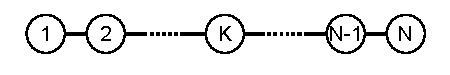
\includegraphics[width=2.5in]{10.matrix3/polymer_linear.pdf}
		\caption{A linear chain of atoms.  The edge atoms interacts with only one neighboring atom.}
		\raisebox{0.8in}{}
		\label{fig:polymer_linear}
	\end{subfigure}
	\begin{subfigure}{0.45\textwidth}
		\centering
		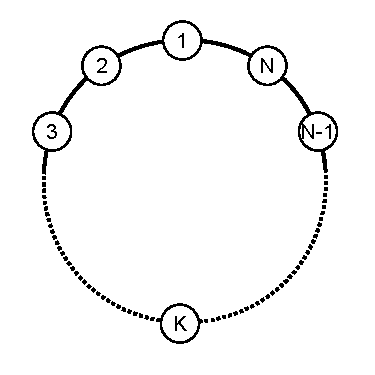
\includegraphics[width=2in]{10.matrix3/polymer_ring.pdf}
		\caption{A circular chain of atoms.  All atoms interacts with two adjacent atoms.}
		\label{fig:polymer_ring}
	\end{subfigure}
\caption{Two different boundary conditions for the chain of atoms.}\label{fig:polymer}
\end{figure}

\noindent
\textbf{A Linear Chain}

\medskip
\noindent
Next example is a popular problem in quantum mechanics.
Consider a linear chain of $N$ atoms shown in Fig \ref{fig:polymer_linear}.  All atoms are identical.  Based on a simple tight-binding model\cite{tight_binding}, the Hamiltonian of the system is a tridiagonal matrix:
\begin{equation}
H=\begin{bmatrix}
\alpha & \beta  &        &         &        &        &  0         \\
\beta  & \alpha & \beta  &         &        &        &            \\
       & \ddots & \ddots & \ddots  &        &        &            \\
       &        & \beta  & \alpha  & \beta  &        &            \\
       &        &        & \ddots  & \ddots & \ddots &            \\  
       &        &        &         & \beta  & \alpha & \beta      \\
    0  &        &        &         &        & \beta  & \alpha   
\end{bmatrix}
\end{equation}
where $\alpha$ and $\beta$ are site energy and hopping matrix element.\cite{tight_binding}
Te orbital energy of electrons in the polymer is determined by the equation
\begin{equation}
H \psi_n = E_n \psi_n
\end{equation}
where $E_n$ and $\psi_n$ are energy and wave function of the electron, respectively.  Mathematically speaking, they are eigenvalue and eigenvector.

This problem can be solved analytically.  For $\alpha=-2$ and $\beta=-1$, $E_n = -4 \sin^2 \left ( \displaystyle\frac{n \pi}{2(N+1)} \right )$.  Program \ref{prog:polymer} tries to get the same result using the QR algorithm.  Form $N=10$, it took 141 iterations. The resulting numerical eigenvalues perfectly agree with the exact solution  Figure \ref{fig:tight_binding1} plots the wavefunctions for the lowest three eigenvalues.  The result resemble to those of the particle in the infinite square well\cite{inf_well}.  In fact, the present model is the discrete version of the infinite square well.

\begin{center}
\begin{minipage}{3in}
\small
\begin{Verbatim}[frame=single]
       numerical    exact
n= 1 : E=-3.9190  (-3.9190)
n= 2 : E=-3.6825  (-3.6825)
n= 3 : E=-3.3097  (-3.3097)
n= 4 : E=-2.8308  (-2.8308)
n= 5 : E=-2.2846  (-2.2846)
n= 6 : E=-1.7154  (-1.7154)
n= 7 : E=-1.1692  (-1.1692)
n= 8 : E=-0.6903  (-0.6903)
n= 9 : E=-0.3175  (-0.3175)
n=10 : E=-0.0810  (-0.0810)
\end{Verbatim}
\normalsize
\end{minipage}
\end{center}

\begin{figure}
	\centering
	\begin{subfigure}{0.45\textwidth}
		\centering
		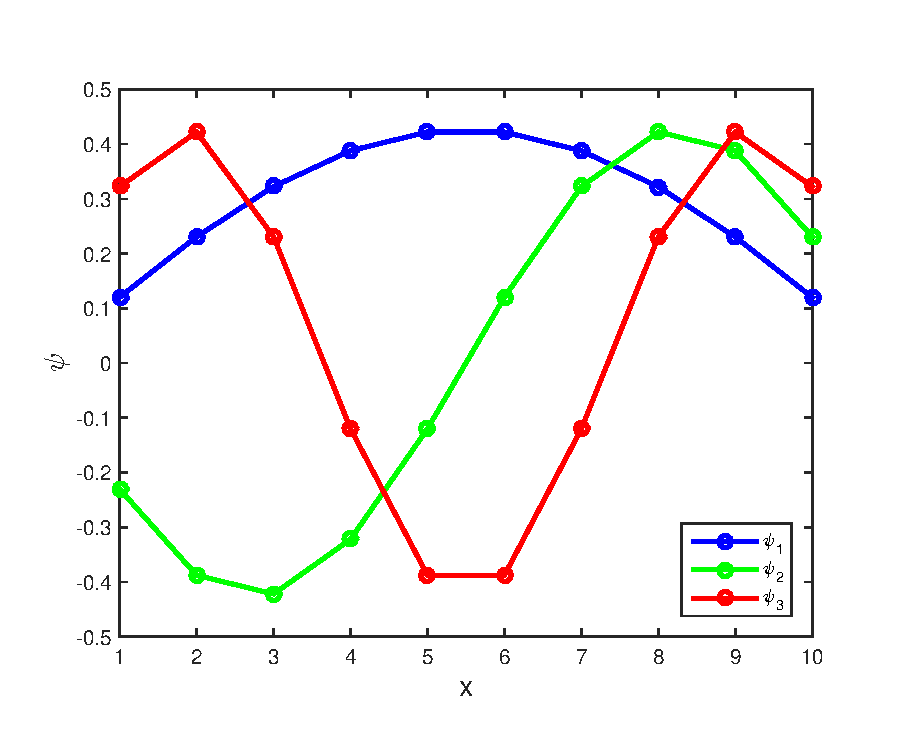
\includegraphics[width=2.5in]{10.matrix3/tight_binding1.pdf}
		\caption{A linear chain of atoms.  The wavefunctions corresponding to the lowest three energy are plotted.}
		\label{fig:tight_binding1}
	\end{subfigure}
	\begin{subfigure}{0.45\textwidth}
		\centering
		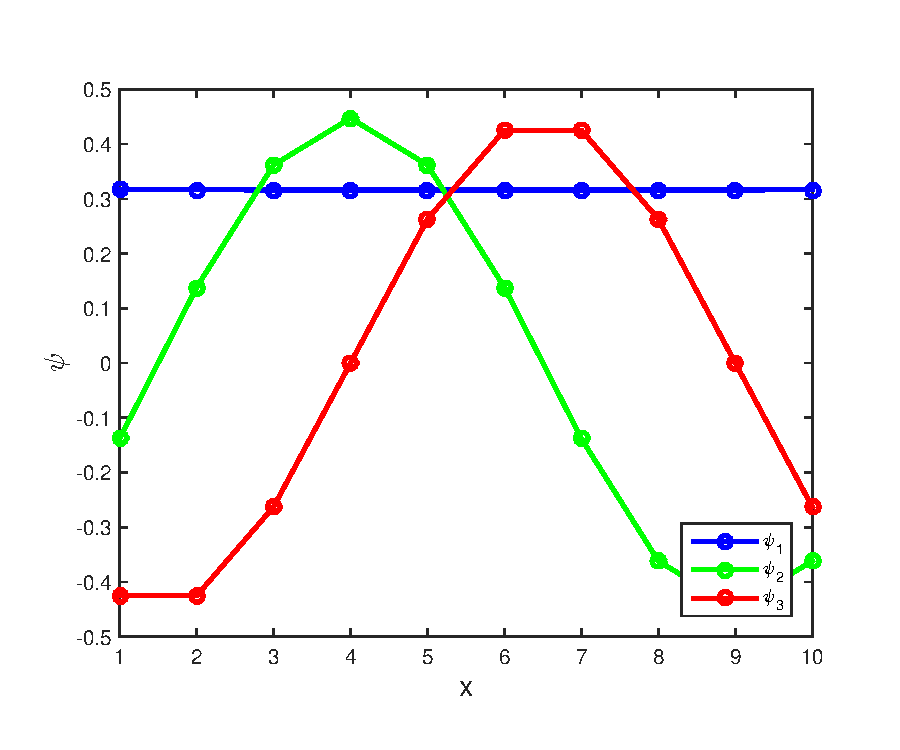
\includegraphics[width=2.5in]{10.matrix3/tight_binding2.pdf}
		\caption{A circular chain of atoms (periodic boundary condition).}
		\label{fig:tight_binding2}
	\end{subfigure}
\caption{Tight binfing model of atomic chains with two different boundary conditions. The wavefunctions corresponding to the lowest three energy are plotted.}
\label{fig:tight_binding}
\end{figure}

\bigskip
\noindent
\textbf{A Circular Chain: Periodic Boundary Condition}

\medskip
\noindent
We continue the previous model of the atomic chain.  This time it is not a linear chain but a ring of atoms (see Fig. \ref{fig:polymer_ring}.  Atom 1 and $N$ are connected so that electron can hop between them. The Hamiltonian is similar to Eq ().  Place $\beta$ at the top-right corner ($H_\textsc{1N}$) and the bottom-left corner ($H_\textsc{N1}$).  The exact solution is $E = \alpha + 2 \beta \cos(2 n \pi/N), n=0, \cdots, N-1$.\cite{tight_binding}  Changing the Hamiltonian in Program \ref{prog:polymer} we obtain the following results.  Again the agreement is perfect.  Note the two-fold degeneracy except for $n=1$ and $n=10$.   This degeneracy is due to the rotational symmetry.  Clockwise and counterclockwise circular motions must have the same energy.  Waveufnctions plotted in  Figure \ref{fig:tight_binding2} illustrates it. The lowest energy state is uniform.  Recalling that the momentum of the particle is proportional to the inverse of the wave function. This state has the infinitely long wavelength and thus the particle must be at rest (in the classical sense).  There is only one such state.  The next two wave functions look like $\sin$ and $\cos$ functions since their phases are shifted by $\pi/2$.  Since they have the same eigenvalue, any linear combination of the two wavefunctions is again the solution.  we can create two traveling waves one in the clockwise and the other in counterclockwise.

\begin{center}
\begin{minipage}{3in}
\small
\begin{Verbatim}[frame=single]
       numerical    exact
n= 1 : E=-4.0000  (-4.0000)
n= 2 : E=-3.6180  (-3.6180)
n= 3 : E=-3.6180  (-3.6180)
n= 4 : E=-2.6180  (-2.6180)
n= 5 : E=-2.6180  (-2.6180)
n= 6 : E=-1.3820  (-1.3820)
n= 7 : E=-1.3820  (-1.3820)
n= 8 : E=-0.3820  (-0.3820)
n= 9 : E=-0.3820  (-0.3820)
n=10 : E= 0.0000  ( 0.0000)
\end{Verbatim}
\normalsize
\end{minipage}
\end{center}

\bigskip
\noindent
\textbf{Impurity in the Chain}

\medskip
\noindent
Previous two examples have simple analytic solutions and thus no numerical calculation is necessary.  However, the agreement between numerical results and exact solutions makes us confident with the numerical methods.  Now, we try a slightly difficult case.
Consider again the chain of atoms shown in Fig. \ref{fig:polymer}.  The $K$-th atom is replaced with an impurity.  Accordingly, the Hamiltonian matrix must be modified.  Assuming that the impurity weakly interacts with the adjacent atoms, we use $H_\textsc{K-1\, K}=
H_\textsc{K,K+1} = -0.1$.  We use Program \ref{prog:polymer} again.  Placing the impurity at $K=3$, we obtain the following eigenvalues.  The exact solution is not known. To see what is happening near the impurity, we plot the wavefunctions of three lowest energy state in Figure \ref{fig:tight_binding3}.  The waveufnctions of the two lowest energy are nearly zero at atoms 1 through 3.  The low energy particle can't hop to the impurity since the hopping matrix element is too small.  It is possible to confine the electron on atom 1 and 2 but that state must have very high energy due to the uncertainty principle. (The momentum becomes large and thus the kinetic energy is also high.).  The third state seems not sensitive to the presence of the impurity.  All higher energy states are only slightly affected by the impurity.

\begin{center}
\begin{minipage}{3in}
\small
\begin{Verbatim}[frame=single]
n= 1 : E=-3.8499
n= 2 : E=-3.4244
n= 3 : E=-3.0526
n= 4 : E=-2.7874
n= 5 : E=-2.1448
n= 6 : E=-1.8552
n= 7 : E=-1.2125
n= 8 : E=-0.9474
n= 9 : E=-0.5756
n=10 : E=-0.1501
\end{Verbatim}
\normalsize
\end{minipage}
\end{center}


\begin{figure}
\centering
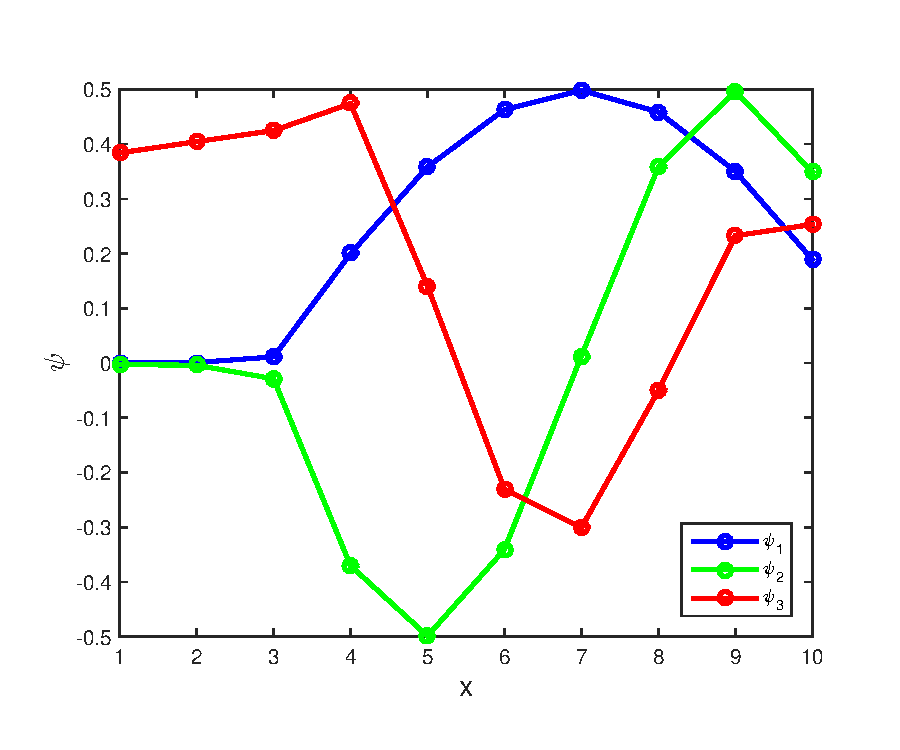
\includegraphics[width=2.5in]{10.matrix3/tight_binding3}
\caption{A chain of atoms with an impurity at $K=3$.  The wavefunctions of  lowest three energy states are plotted.  Note that electrons in the lowest two energy states do not hop to atom 1 and 2.  The impurity seems blocking it.} 
\label{fig:tight_binding3}
\end{figure}

\exercise
What will happen if the hopping matrix elements between the impurity and its neighbors are bigger than other hopping matrix elements?


\newpage
\section{Problems}

\begin{enumerate}[labelwidth=0.5cm,labelindent=0cm,leftmargin=*,label=\bfseries \thechapter.\arabic*,align=left]

\item A Triangular Molecule

\begin{minipage}{4.5in}
Consider a triangular molecule consisting of three identical atoms as shown in Figure. A simple model assume that electrons are hopping between potential wells, $V_n$ ($n$=1,2,3).
The distance between spheres is short enough for
electrons to jump from one well to another.  Following a tight-binding method,
we use a basis, $\ket{\psi_n}$ 
representing an electron in the potential well $V_n$ .  Using this base set, the Hamiltonian of the system can be written in a matrix form as
\begin{equation}
H  = 
\begin{bmatrix}
\epsilon & \beta & \beta \\
\beta & \epsilon & \beta \\
\beta & \beta & \epsilon
\end{bmatrix}
\end{equation}
\end{minipage}
\begin{minipage}{1.9in}
\hfill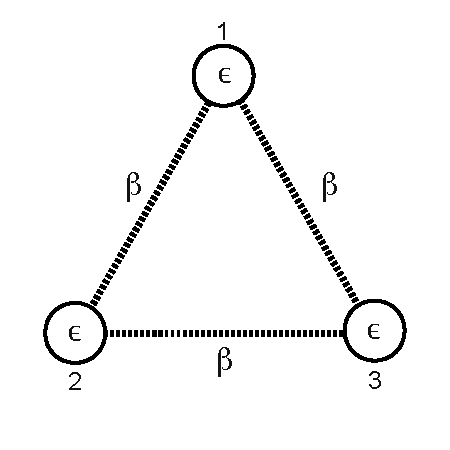
\includegraphics[width=1.5in]{10.matrix3/trimer.pdf} 
\end{minipage}
where $\epsilon$ and $\beta_i$ denote the energy of an electron trapped
in a potential well and a hopping matrix element between the potential wells,
respectively.  Here we assume $\epsilon < 0$ and $\beta < 0$. 

A state of the particle is given by a column vector
\begin{equation}
\mathbf{u} = 
\begin{bmatrix}
u_1 \\ u_2 \\ u_3
\end{bmatrix}
\end{equation}
Energy eigenstates are determined by Schr\"{o}nger equation
\begin{equation}
H \mathbf{u} = E \mathbf{u}
\end{equation}
which is an eigenvalue problem. We want to find all eigenvalues using the QR method.  We can use Program \ref{prog:qr_eigen}.
Assuming that $\epsilon=-2$ and $\beta=-1$, the exact solutions are $\lambda_1 = -4$ and $\lambda_2=\lambda_3=-1$.  The corresponding eigenvectors are
\begin{equation}
\mathbf{x}_1 = \begin{bmatrix} \frac{1}{\sqrt{3}} \\ \frac{1}{\sqrt{3}} \\ \frac{1}{\sqrt{3}} \end{bmatrix}, \quad 
\mathbf{x}_2 = \begin{bmatrix} \frac{1}{\sqrt{2}} \\ -\frac{1}{\sqrt{2}} \\ 0  \end{bmatrix}, \quad
\mathbf{x}_3 = \begin{bmatrix} -\frac{1}{\sqrt{6}} \\-\frac{1}{\sqrt{6}} \\ \frac{2}{\sqrt{6}} \end{bmatrix} 
\end{equation} 

Find numerically the all eigenvalues and the corresponding eigenvectors.  Compare the results with the exact values.
\end{enumerate}

\newpage

\noindent
\section*{MATLAB Source Codes}
\addcontentsline{toc}{section}{\protect\numberline{}MATLAB Source Codes}

\bigskip
\noindent
\program
\label{prog:power_eigen}
\footnotesize
\begin{verbatim}
%%*************************************************************************
%*     Example 10.1 - 10.3                                                *
%*     filename: ch10pr01.m                                               *
%*     program listing number: 10.1                                       *
%*                                                                        *
%*     This program finds eigenvalues and eigenvectors of a symmetric     *
%*     matrix using the power method.                                     *
%*                                                                        *
%*     Programmed by Ryoichi Kawai for Computational Physics Course.      *
%*     Last modification:  01/08/2013.                                    *
%**************************************************************************
clear all;

% system
A=[[2,1,0];[1,2,1];[0,1,2]];
% A=inv(A);                     % Example 9.2
% lambda0=1.5;                  % Example 9.3
% A=inv(A-lambda0*eye(3,3));    % Example 9.3



% tolerance
tol = 1e-7;
found=false;
n=1;

% initial guess
x=rand(3,1);
x=[2;-sqrt(2);0]; 

% normalization
u0=x/sqrt((x'*x));

% power method iteration
while not(found)
    x=A*x;   % update x
    u1=x/sqrt(x'*x);   % normalization
    err=sqrt( (u1-u0)'*(u1-u0) );   %error
    if err < tol
        found=true;
    else
        u0=u1;
        n=n+1;
    end
end

% eigenvalue
lambda=u1'*A*u1;
lambda=1/lambda;             % Example 9.2       
%lambda = lambda0+1/lambda;  % Example 9.3

fprintf('Eigenvalue=%.6f \n',lambda)
fprintf('Eigenvector\n');
fprintf('%.6f\n',u1);
\end{verbatim}
\normalsize

\ruleend
\bigskip
\noindent
\program
\label{prog:inverse_eigen}
\footnotesize
\begin{verbatim}
%**************************************************************************
%*     Example 10.4                                                       *
%*     filename: ch10pr02.m                                               *
%*     program listing number: 10.2                                       *
%*                                                                        *
%*     This program finds eigenvalues and eigenvectos of a symmetric      *
%*     matrix using the inverse iteration method method.                  *
%*                                                                        *
%*     Programed by Ryoichi Kawai for Computational Physics Course.       *
%*     Last modification:  01/08/2013.                                    *
%**************************************************************************
clear all;

% Matrix
A=[[2,1,0];[1,2,1];[0,1,2]];


for i=1:6;
    % generate an initial guess
    if i<4
       q=0.5*i;
    else
       q=0.5*(i+1);
    end
    
% tolerance
tol = 1e-7;

found=false;
n=1;

% Generate a random vector
b0=rand(3,1);
b0=b0/sqrt(b0'*b0);

B=A-q*eye(3,3);

% inverse iteration method
while not(found) 
    y=gauss(B,b0);  % solve linear equation by the Gaussian elimination
    b1=y/sqrt(y'*y);
    if b1(1)<0 % correct the phase.
        b1=-b1;
    end
    err=sqrt( (b1-b0)'*(b1-b0) ); 
    if err < tol
        found=true;
    else
        b0=b1;
        n=n+1;
    end
end

% eigenvalue
lambda=(b1'*A*b1);
fprintf('Guess=%.3f,   Eigenvalue=%.6f \n',q,lambda)

end
\end{verbatim}
\normalsize

\ruleend
\bigskip
\noindent
\program
\label{prog:jacobi_eigen}
\footnotesize
\begin{verbatim}
%**************************************************************************
%*     Example 10.5                                                       *
%*     filename: ch10pr03.m                                               *
%*     program listing number: 10.3                                       *
%*                                                                        *
%*     This program finds eigenvalues and eigenvectors of a symmetric     *
%*     matrix using the Jacobi transformation method.                     *
%*                                                                        *
%*     Programmed by Ryoichi Kawai for Computational Physics Course.      *
%*     Last modification:  02/08/2015.                                    *
%**************************************************************************
clear all

% Define the matrix
A=[[1,-4,2];[-4,1,-2];[2,-2,-2]];

% Tolerance
tol = 1e-4;

% Evalkuate error
S=0;
for i=1:3
    for j=i+1:3
        S=S+A(i,j)^2;
    end
end

P=eye(3,3); %Initial transformation matrix

while S > tol
    for i=1:3
        for j=i+1:3
            if A(i,j) ~= 0
                % Jacobian rotation
                if A(j,j)==A(i,i)
                    c=-1/sqrt(2);
                    s=-1/sqrt(2);
                else
                    beta=(A(j,j)-A(i,i))/(2*A(i,j));
                    t=sign(beta)/(abs(beta)+sqrt(beta^2+1));
                    c=1/sqrt(t^2+1);
                    s=t/sqrt(t^2+1);
                end
                r=s/(1+c);
                ai = c^2*A(i,i)+s^2*A(j,j)-2*s*c*A(i,j);
                aj = s^2*A(i,i)+c^2*A(j,j)+2*s*c*A(i,j);
                A(i,i)=ai;
                A(j,j)=aj;
                % Transformation matrix
                Q=eye(3,3);
                Q(i,i)=c;
                Q(j,j)=c;
                Q(i,j)=s;
                Q(j,i)=-s;
                P=P*Q;
                for k=1:3
                    if k~=i && k~=j
                        aki=c*A(k,i)-s*A(k,j);
                        akj=c*A(k,j)+s*A(k,i);
                        A(k,i)=aki;
                        A(i,k)=aki;
                        A(k,j)=akj;
                        A(j,k)=akj;
                    end
                end
                A(i,j)=0;
                A(j,i)=0;
            end
        end
    end
    
    % Evaluate error
    S=0;
    for i=1:3
        for j=i+1:3
            S=S+abs(A(i,j));
        end
    end
end

fprintf('\nTransformed Matrix\n')
fprintf('%8.4f  %8.4f  %8.4f\n',A')

fprintf('\nTransformation Matrix\n')
fprintf('%8.4f  %8.4f  %8.4f\n',P')
\end{verbatim}
\normalsize

\ruleend
\bigskip
\noindent
\program
\label{prog:qr_eigen}
\footnotesize
\begin{verbatim}
%**************************************************************************
%*     Example 10.6                                                       *
%*     filename: ch10pr04.m                                               *
%*     program listing number: 10.4                                       *
%*                                                                        *
%*     This program finds eigenvalues and eigenvectos of a symmetric      *
%*     matrix using the QR algorithm method.                              *
%*                                                                        *
%*     Uses MATLAB function qr()                                          *
%*                                                                        *
%*     Programmed by Ryoichi Kawai for Computational Physics Course.      *
%*     Last modification:  02/08/2015.                                    *
%**************************************************************************
clear all

% Define the matrix
A=[[1,-4,2];[-4,1,-2];[2,-2,-2]];

% Tolerance
tol = 1e-8;

% Magnitude of total off-diagonal elements
S=0;
for i=1:3
    for j=i+1:3
        S=S+A(i,j)^2;
    end
end

P=eye(3,3);
while S > tol
    [Q, R] =qr(A);  % QR decomposition
    A = R*Q; % Orthogonal transformation
    P=P*Q;   % Accumulating the transformation
    % Error evaluation
    S=0;
    for i=1:3
        for j=i+1:3
            S=S+A(i,j)^2;
        end
    end
end

fprintf('# of iterations = %d\n',n)

fprintf('\nTransformed Matrix\n')
fprintf('%8.4f  %8.4f  %8.4f\n',A')

fprintf('\nTransformation Matrix\n')
fprintf('%8.4f  %8.4f  %8.4f\n',P')   
\end{verbatim}
\normalsize

\ruleend
\bigskip
\noindent
\program
\label{prog:eigenmodes}
\footnotesize
\begin{verbatim}
%**************************************************************************
%*     Section 10.5.1                                                     *
%*     filename: ch10pr05.m                                               *
%*     program listing number: 10.5                                       *
%*                                                                        *
%*     This program finds eigen modes of   harmonic oscillators.          *
%*     The highest and lowest frequencies are obtained by the power       *
%*     method and the remaining frequency is computed by the inverse      *
%*     iteration method.                                                  *
%*                                                                        *
%*     Programmed by Ryoichi Kawai for Computational Physics Course.      *
%*     Last modification:  02/08/2015.                                    *
%**************************************************************************
clear all;

% system parameters
k1=2; k2=4; k3=4; k4=2;
m1=2; m2=4; m3=3;
K=[[k1+k2, -k2, 0];[-k2,k2+k3,-k3];[0,-k3,k3+k4]];
Minv=[[1/m1,0,0];[0,1/m2,0];[0,0,1/m3]];
A0=Minv*K;

tol = 1e-7; % tolerance

% Find the largest/smallest eigenvalues
% by the power method.
for i=1:2 

    if i==1
        A=A0;  % for largest eigenvalue
    else
        A=inv(A0); % for smallest
    end

    found=false;
    n=1;
    
    x=rand(3,1); % initial guess
    u0=x/sqrt((x'*x)); % normalization

% power method iteration
    while not(found)
        x=A*x;   % update x
        u1=x/sqrt(x'*x);   % normalization
        err=sqrt( (u1-u0)'*(u1-u0) );   %error
        if err < tol
            found=true;
        else
            u0=u1;
            n=n+1;
        end
    end

    if i==1
        lambda(1)=u1'*A*u1; % largest eigenvalue
        u(1:3,1)=u1;
    else
        lambda(3)=1/(u1'*A*u1); % smallest
        u(1:3,3)=u1;
    end 
end

% The other eigenvalue by the inverse 
% iterative method.
% guess=middle between the largest and
% the lowest.
q = (lambda(1)+lambda(2))/2; 
A = A0;

b0=rand(3,1); % random vector
b0=b0/sqrt(b0'*b0);
B=A-q*eye(3,3); % shifted matrix

found=false;
n=1;

% inverse iteration method
while not(found) 
    y=gauss(B,b0);
    b1=y/sqrt(y'*y);
    if b1(1)<0 % correct the phase.
        b1=-b1;
    end
    err=sqrt( (b1-b0)'*(b1-b0) ); 
    if err < tol
        found=true;
    else
        b0=b1;
        n=n+1;
    end
end

% eigenvalue
lambda(2)=(b1'*A*b1);
u(1:3,2)=b1;

% output
for i=1:3
    fprintf('\nFrequency=%.6f \n',sqrt(lambda(i)))
    fprintf('Eigenvector\n');
    fprintf('%.6f\n',u(:,i));
end
\end{verbatim}
\normalsize

\ruleend
\bigskip
\noindent
\program
\label{prog:polymer}
\footnotesize
\begin{verbatim}
%**************************************************************************
%*     Section 10.5.2 - 10.5.4                                            *
%*     filename: ch10pr06.m                                               *
%*     program listing number: 10.6                                       *
%*                                                                        *
%*     This program finds energy and wavefunction of a chain of atoms     *
%*     using the QR algorithm method.                                     *
%*                                                                        *
%*     Uses MATLAB function qr()                                          *
%*                                                                        *
%*     Programmed by Ryoichi Kawai for Computational Physics Course.      *
%*     Last modification:  02/09/2015.                                    *
%**************************************************************************
clear all
%
N=10;
alpha=-2;
beta=-1;

% Define the matrix
A=zeros(N,N);

for i=1:N
    A(i,i)=alpha;
end

for i=1:N-1
    j=i+1;
    A(i,j)=beta;
    A(j,i)=beta;
end   

% Tolerance
tol = 1e-8;

% Magnitude of total off-diagonal elements
S=0;
for i=1:N
    for j=1:i-1
        S=S+A(i,j)^2;
    end
end

P=eye(N,N);
n=0;
while S > tol
    n=n+1;
    [Q, R] =qr(A);  % QR decomposition
    A = R*Q; % Orthogonal transformation
    P=P*Q;   % Accumulating the transformation
    % Error evaluation
    S=0;
    for i=1:N
        for j=1:i-1
            S=S+A(i,j)^2;
        end
    end
end

fprintf('# of iterations = %d\n',n)

fprintf('Eigenvalues\n')
for n=1:N
    E=-4*sin((N-n+1)*pi/(2*(N+1)))^2;
    fprintf('n=%2d : E=%6.4f  (%6.4f)\n',n,A(n,n),E)
end

fprintf('\nTransformation Matrix\n')
P

p=plot([1:N],P(:,1),'-o',[1:N],P(:,2),'-o',[1:N],P(:,3),'-o');
set(p(1),'linewidth',2,'color','blue')
set(p(2),'linewidth',2,'color','green')
set(p(3),'linewidth',2,'color','red')
xlabel('x','fontsize',14)
ylabel(texlabel('psi'),'fontsize',14)
legend(p,{texlabel('psi_1'),texlabel('psi_2'),texlabel('psi_3')});
legend(p,'Location','SouthEast');

\end{verbatim}
\normalsize

\ruleend

\bigskip
\noindent
\section*{Python Source Codes}
\addcontentsline{toc}{section}{\protect\numberline{}Python Source Codes}
\setcounter{program}{0}


\bigskip
\noindent
\program
\footnotesize
\begin{verbatim}
#!/usr/bin/env python3
# -*- coding: utf-8 -*-
"""
%**************************************************************************
%*     Example 10.1 -10.3                                                 *
%*     filename: ch10pr01.m                                               *
%*     program listing number: 10.1                                       *
%*                                                                        *
%*     This program finds eigenvalues and eigenvectos of a 3x3symmetric   *
%*     matrix using the power method.                                     *
%*                                                                        *
%*     Programed by Ryoichi Kawai for Computational Physics Course.       *
%*     Last modification:  01/08/2013.                                    *
%**************************************************************************
"""
import numpy as np

def evpower(A):

    # tolerance
    tol=1.0e-7
    found=False

    # create arrays
    u0=np.matrix(np.zeros(3)).transpose()
    u1=np.matrix(np.zeros(3)).transpose()

    # initial guess
    x=np.matrix(np.random.rand(3)).transpose()

    # normalization
    u0=x/np.sqrt(np.asscalar(x.transpose()*x))

    # power method iteration
    n=0
    while not(found):
        x=A*x   # update x
        u1=x/np.sqrt(np.asscalar(x.transpose()*x))   # normalization
        err=np.sqrt( np.asscalar((u1-u0).transpose()*(u1-u0)) )   #error
        if err < tol:
            found=True
        else:
            u0[:]=u1[:]

        n+=1
        
    eig=np.asscalar(u1.transpose()*A*u1) 
    
    return [n, eig, u1]
        
A=np.matrix([[2.,1.,0.],[1.,2.,1.],[0.,1.,2.]])

# SOlution by eignvalue solver in numpy
eig_np, u_np = np.linalg.eig(A)

# Example 10.1
[n, eig, u] = evpower(A)
# Eigenvalue

print('\nLargest Eigenvalue (Example 10.1)')
print('Iteration=',n)
print('Eigenvale={0:f} (numpy: {1:f})'.format(eig, eig_np[0]))
print('Eigenvector=[{0:8.4f}, {1:8.4f}, {2:8.4f}]'\
                    .format(u[0,0],u[1,0],u[2,0]))
print('    (numpy):[{0:8.4f}, {1:8.4f}, {2:8.4f}]'\
      .format(u_np[0,0],u_np[1,0],u_np[2,0]))
eig_max=eig

# Example 10.2
A=np.matrix([[2.,1.,0.],[1.,2.,1.],[0.,1.,2.]])
A=np.linalg.inv(A)
[n, eig, u] = evpower(A)
# Eigenvalue
eig=1.0/eig

print('\nSmallest Eigenvalue (Example 10.2)')
print('Iteration=',n)
print('Eigenvale={0:f} (numpy: {1:f})'.format(eig, eig_np[2]))
print('Eigenvector=[{0:8.4f}, {1:8.4f}, {2:8.4f}]'\
                    .format(u[0,0],u[1,0],u[2,0]))
print('    (numpy):[{0:8.4f}, {1:8.4f}, {2:8.4f}]'\
      .format(u_np[0,2],u_np[1,2],u_np[2,2]))
eig_min=eig

# Example 10.3
A=np.matrix([[2.,1.,0.],[1.,2.,1.],[0.,1.,2.]])
eig0=0.5*(eig_min+eig_max)

A=np.linalg.inv(A-eig0*np.identity(3))
[n, eig, u] = evpower(A)
eig=1.0/eig+eig0

print('\nThe Eigenvalue between the smallest and largest (Example 10.3)')
print('Iteration=',n)
print('Eigenvale={0:f} (numpy: {1:f})'.format(eig, eig_np[1]))
print('Eigenvector=[{0:8.4f}, {1:8.4f}, {2:8.4f}]'\
                    .format(u[0,0],u[1,0],u[2,0]))
print('    (numpy):[{0:8.4f}, {1:8.4f}, {2:8.4f}]'\
      .format(u_np[0,1],u_np[1,1],u_np[2,1]))
\end{verbatim}
\normalsize

\ruleend

\bigskip
\noindent
\program
\footnotesize
\begin{verbatim}
#!/usr/bin/env python3
# -*- coding: utf-8 -*-
"""
%**************************************************************************
%*     Example 10.4                                                       *
%*     filename: ch10pr02.py                                              *
%*     program listing number: 10.2                                       *
%*                                                                        *
%*     This program finds eigenvalues and eigenvectos of a symmetric      *
%*     matrix using the inverse iteration method method.                  *
%*                                                                        *
%*     Programed by Ryoichi Kawai for Computational Physics Course.       *
%*     Last modification:  02/17/2017.                                    *
%**************************************************************************
"""
import numpy as np

# Set a matrix
A=np.matrix([[2,1,0],[1,2,1],[0,1,2]])

for q in (0.5,1.0,1.5,2.5,3.0,3.5):
    
    #tolerance
    tol = 1e-7

    found=False
    n=1

    # Generate a random vector
    b0=np.random.rand(3,1)
    b0=b0/np.linalg.norm(b0)

    B=A-q*np.identity(3)

    # inverse iteration method
    while not(found):
        y=np.linalg.solve(B,b0)
        b1=y/np.linalg.norm(y)
        if b1[0]<0: # correct the phase.
            b1=-b1

        err=np.linalg.norm(b1-b0)
        if err < tol:
            found=True
        else:
            b0=b1
            n+=1

    # eigenvalue
    eig= np.asscalar(b1.transpose()*A*b1)
    print('Guess={0:6.3f},   Eigenvalue={1:10.6f}'.format(q,eig))
\end{verbatim}
\normalsize

\ruleend

\bigskip
\noindent
\program
\footnotesize
\begin{verbatim}
#!/usr/bin/env python3
# -*- coding: utf-8 -*-
"""
%**************************************************************************
%*     Example 10.5                                                       *
%*     filename: ch10pr03.m                                               *
%*     program listing number: 10.3                                       *
%*                                                                        *
%*     This program finds eigenvalues and eigenvectos of a symmetric      *
%*     matrix using the Jacobi transformation method.                     *
%*                                                                        *
%*     Programed by Ryoichi Kawai for Computational Physics Course.       *
%*     Last modification:  02/08/2015.                                    *
%**************************************************************************
"""
import numpy as np

# Define the matrix
A=np.matrix([[1.,-4.,2.],[-4.,1.,-2.],[2.,-2.,-2.]])

# Tolerance
tol=1.0e-4

# Evaluate error
S=0.0
for i in range(0,3):
    for j in range(i+1,3):
        S=S+abs(A[i,j])

# Initial transformation matrix
P=np.matrix(np.identity(3))

while S > tol:
    for i in range(0,3):
        for j in range(i+1,3):
            if A[i,j] != 0:
                # Jacobian rotation
                if A[j,j]==A[i,i]:
                    c=-1./np.sqrt(2.)
                    s=-1./np.sqrt(2.)
                else:
                    beta=(A[j,j]-A[i,i])/(2.0*A[i,j])
                    t=np.sign(beta)/(np.abs(beta)+np.sqrt(beta**2+1.0))
                    c=1./np.sqrt(t**2+1.0)
                    s= t/np.sqrt(t**2+1.0)

                r=s/(1.0+c)
                ai = c**2*A[i,i]+s**2*A[j,j]-2.0*s*c*A[i,j]
                aj = s**2*A[i,i]+c**2*A[j,j]+2.0*s*c*A[i,j]
                A[i,i]=ai
                A[j,j]=aj
                # Transformation matrix
                Q=np.matrix(np.identity(3))
                Q[i,i]=c
                Q[j,j]=c
                Q[i,j]=s
                Q[j,i]=-s
                P=P*Q

                for k in range(0,3):
                    if k!=i and k!=j:
                        aki=c*A[k,i]-s*A[k,j]
                        akj=c*A[k,j]+s*A[k,i]
                        A[k,i]=aki
                        A[i,k]=aki
                        A[k,j]=akj
                        A[j,k]=akj

                A[i,j]=0.0
                A[j,i]=0.0

    # Evaluate error
    S=0.0
    for i in range(0,3):
        for j in range(i+1,3):
            S=S+abs(A[i,j])

print('\nTransformed Matrix\n')
print(A)

print('\nTransformation Matrix\n')
print(P)
\end{verbatim}
\normalsize

\ruleend

\bigskip
\noindent
\program
\footnotesize
\begin{verbatim}
#!/usr/bin/env python3
# -*- coding: utf-8 -*-
"""
%**************************************************************************
%*     Example 10.6                                                       *
%*     filename: ch10pr04.py                                              *
%*     program listing number: 10.4                                       *
%*                                                                        *
%*     This program finds eigenvalues and eigenvectos of a symmetric      *
%*     matrix using the QR algorithm method.                              *
%*                                                                        *
%*     Uses NUMPY function qr()                                           *
%*                                                                        *
%*     Programed by Ryoichi Kawai for Computational Physics Course.       *
%*     Last modification:  02/18/2017.                                    *
%**************************************************************************
"""
import numpy as np

# Define the matrix
A=np.matrix([[1.,-4.,2.],[-4.,1.,-2.],[2.,-2.,-2.]])

# Tolerance
tol = 1e-8;

# Magnitude of total off-diagonal elemens
S=0.0
for i in range(0,3):
    for j in range(i+1,3):
        S=S+A[i,j]**2

# Initial transformation matrix
P=np.matrix(np.identity(3))

n=0
while S > tol:
    n+=1
    [Q, R] =np.linalg.qr(A)  # QR decomposition
    A=R*Q  # Orthogonal transformation
    P=P*Q  # Accumulating the transformation
    # Error evaluation
    S=0.0
    for i in range(0,3):
        for j in range(i+1,3):
            S=S+A[i,j]**2

print('# of iterations ={0:d}'.format(n))

print('\nTransformed Matrix\n')
print(A)

print('\nTransformation Matrix\n')
print(P)
\end{verbatim}
\normalsize

\ruleend

\bigskip
\noindent
\program
\footnotesize
\begin{verbatim}
#!/usr/bin/env python3
# -*- coding: utf-8 -*-
"""
%**************************************************************************
%*     Section 10.5.1                                                     *
%*     filename: ch10pr05.py                                              *
%*     program listing number: 10.5                                       *
%*                                                                        *
%*     This program finds eigenmodes of cpoupled harmonic oscillators.    *
%*     The higest and lowest frequencies are obgtained by the power       *
%*     method and the remaining frequency is computed by the inverse      *
%*     iteration method.                                                  *
%*                                                                        *
%*     Programed by Ryoichi Kawai for Computational Physics Course.       *
%*     Last modification:  02/18/2017.                                    *
%**************************************************************************
"""
import numpy as np

# system parameters
k1=2.0; k2=4.0; k3=4.0; k4=2.0
m1=2.0; m2=4.0; m3=3.0
K=np.matrix([[k1+k2, -k2, 0.0],[-k2,k2+k3,-k3],[0.0,-k3,k3+k4]])
Minv=np.matrix([[1.0/m1,0.0,0.0],[0.0,1.0/m2,0.0],[0.0,0.0,1/m3]])
A0=Minv*K
A=np.matrix(np.zeros((3,3)))
u=np.matrix(np.zeros((3,3)))
eig=np.zeros(3)

tol = 1e-7 # tolerance

# Find the largest/smallest eigenvalues
# by the power method.
for i in (0,1,2):

    if i==0:
        A[:,:]=A0[:,:]  # for largest eigenvalue
    else:
        A=np.linalg.inv(A0) # for smallest

    found=False
    x=np.matrix(np.random.rand(3)).transpose()    # initial guess
    u0=x/np.linalg.norm(x)  # normalization

# power method iteration
    n=1
    while not(found):
        x=A*x   # update x
        u1=x/np.linalg.norm(x)   # normalization
        err=np.linalg.norm(u1-u0)   # error
        if err < tol:
            found=True
        else:
            u0=u1
            n+=1

        if i==0:
            eig[0]=u1.transpose()*A*u1 # largest eigenvalue
            u[:,0]=u1
        else:
            eig[2]=1.0/(u1.transpose()*A*u1) # smallest
            u[:,2]=u1

# The other eigenvalue by the inverse 
# iterative method.
# guess=middle between the largest and
# the lowest.

u0=np.matrix(np.random.rand(3)).transpose() # random vector
u0=u0/np.linalg.norm(u0)
q = (eig[0]+eig[2])/2.0 
A=A0-q*np.identity(3)  # shifted matrix

found=False
n=1

# inverse iteration method
while not(found):
    x=np.linalg.solve(A,u0)
    u1=x/np.linalg.norm(x)
    if u1[0]<0:  # correct the phase.
        u1=-u1

    err=np.linalg.norm(u1-u0) 
    if err < tol:
        found=True
    else:
        u0=u1
        n+=1

# eigenvalue
eig[1]=u1.transpose()*A0*u1
u[:,1]=u1

# output
for i in range(0,3):
    print('\nFrequency={0:f}'.format(np.sqrt(eig[i])))
    print('Eigenvector')
    print(u[:,i])
\end{verbatim}
\normalsize

\ruleend

\bigskip
\noindent
\program
\footnotesize
\begin{verbatim}
#!/usr/bin/env python3
# -*- coding: utf-8 -*-
"""
%**************************************************************************
%*     Section 10.5.2 - 10.5.4                                            *
%*     filename: ch10pr06.py                                              *
%*     program listing number: 10.6                                       *
%*                                                                        *
%*     This program finds energy and wavefunction of a chain of atoms     *
%*     using the QR algorithm method.                                     *
%*                                                                        *
%*     Uses NUMPY method qr()                                             *
%*                                                                        *
%*     Programed by Ryoichi Kawai for Computational Physics Course.       *
%*     Last modification:  02/18/2017.                                    *
%**************************************************************************
"""
import numpy as np
import matplotlib.pyplot as plt

N=10  # The size of the chain molecule
alpha=-2.0
beta=-1.0

# Define the tridiagonal matrix
A=np.zeros((N,N))
for i in range(0,N):
    A[i,i]=alpha
for i in range(0,N-1):
    A[i,i+1]=beta
    A[i+1,i]=beta
A=np.matrix(A)

# Tolerance
tol = 1.0e-8

# Magnitude of total off-diagonal elemens
S=0.0
for i in range(0,N):
    for j in range(0,i):
        S=S+A[i,j]**2

P=np.matrix(np.identity(N))

n=0
while S > tol:
    n+=1
    Q, R=np.linalg.qr(A);  # QR decomposition
    A=R*Q  #Orthogonal transformation
    P=P*Q    #Accumulating the transformation
    # Error evaluation
    S=0.0
    for i in range(0,N):
        for j in range(0,i):
            S=S+A[i,j]**2

print('# of iterations={0:d}'.format(n))
print('Eigenvalues\n')
for n in range(0,N):
    E=-4.*np.sin((N-n)*np.pi/(2*(N+1)))**2
    print('n={0:d} : E={1:f} ({2:f})'.format(n,A[n,n],E))

print('\nTransformation Matrix\n')
print(P)

plt.figure(figsize=(6,5))
plt.plot(np.linspace(0,N-1,N),P[:,0],'-ob',label=r'$\psi_1$')
plt.plot(np.linspace(0,N-1,N),P[:,1],'-og',label=r'$\psi_2$')
plt.plot(np.linspace(0,N-1,N),P[:,2],'-or',label=r'$\psi_3$')

plt.xlabel('x',fontsize=14)
plt.ylabel(r'$\psi$',fontsize=14)
plt.legend(loc=4)
plt.show()
\end{verbatim}
\normalsize

\ruleend
\newpage
%\chapbibliography
\bibliographystyle{unsrt}
\bibliography{compphys}